\documentclass{article}

\usepackage{caption}
\usepackage{subcaption}
\usepackage{amsmath}
\usepackage{url}

\usepackage{arxiv}

\usepackage[utf8]{inputenc} % allow utf-8 input
\usepackage[T1]{fontenc}    % use 8-bit T1 fonts
\usepackage{hyperref}       % hyperlinks
\usepackage{url}            % simple URL typesetting
\usepackage{booktabs}       % professional-quality tables
\usepackage{amsfonts}       % blackboard math symbols
\usepackage{nicefrac}       % compact symbols for 1/2, etc.
\usepackage{microtype}      % microtypography
\usepackage{lipsum}
\usepackage{graphicx}

\usepackage{algorithm2e}

\usepackage[backend=biber]{biblatex}
\addbibresource{refs.bib}

\graphicspath{ {./fig/} }

\usepackage{tikz}
\usetikzlibrary{arrows.meta, bending, positioning}

\newcommand{\map}{\mathop{\bigoplus}\limits}
\newcommand{\txtop}[1]{\mathop{\mathtt{#1}}\limits}

\newcommand{\expr}{\txtop{expression}}

\newcommand{\fn}{\txtop{function}}
\newcommand{\tanhl}{\txtop{tanh}}
\newcommand{\linear}{\txtop{linear}}
\newcommand{\sigmoid}{\txtop{sigmoid}}
\newcommand{\argmin}{\txtop{argmin}}
\newcommand{\ntos}{\txtop{noise2self}}

\newcommand{\DeePWAK}{\txtop{DeePWAK}}
\newcommand{\encoder}{\txtop{encoder}}
\newcommand{\decoder}{\txtop{decoder}}
\newcommand{\partitioner}{\txtop{partitioner}}


\SetKwProg{Fn}{Function}{}{end}
\SetKwProg{Dat}{Data}{}{end}

\SetKwInOut{Hyper}{Hyperparameters}

\SetKwFunction{softmax}{softmax}
\SetKwFunction{MSE}{MSE}
\SetKwFunction{transpose}{transpose}
\SetKwFunction{matmul}{matmul}
\SetKwFunction{eucl}{euclidean}
\SetKwFunction{pca}{pca}
\SetKwFunction{knn}{knn}

\SetKwFunction{sample}{sample}
\SetKwFunction{loss}{loss}
\SetKwFunction{train}{train}
\SetKwFunction{WAK}{WAK}
\SetKwFunction{DEWAKSS}{DEWAKSS}
\SetKwFunction{DeePWAKBlock}{DeePWAKBlock}
\SetKwFunction{DeePWAK}{DeePWAK}

\SetKwFunction{Type}{Type}
\SetKwFunction{List}{List}
\SetKwFunction{Arch}{Arch}
\SetKwFunction{Params}{Params}
\SetKwFunction{Model}{Model}
\SetKwFunction{Linear}{Linear}
\SetKwFunction{Partitioner}{Partitioner}

\date{\today}

\title{Denoising with a Partitioned Affinity Kernel Allows Efficient End-to-End Differentiable Clustering}

\author{
  Keira Wiechecki \\
  %Center for Genomics \& Systems Biology \\
  %New York University \\
  \And
  Jade Zaslavsky
  \And
  Margaux Failla
  \And
  Lionel Christiaen \\
}

\begin{document}
\maketitle

\begin{abstract}
Here we introduce Denoising by Deep learning of a Partitoned Weighted Affinity Kernel (DeePWAK). 
\end{abstract}

\section{Introduction}
  %Clustering is a special case of sparse dictionary learning where all features are discrete.
Fundamentally, unsupervised learning is a problem of finding the latent space of a data set.
Denoising, compression, and clustering all ultimately attempt to solve this problem, but approach it from different directions.
Denoising aims to remove spurious dimensions whereas compression looks to select informative dimensions.
The connection to clustering is less obvious, but no less foundational\cite{9830658}.


At its heart, clustering is an optimization problem of how to partition a data set given some loss function.

There are a few ways to conceptualize this isomorphism.

\paragraph{Clustering as principal components in latent space}
Data are sparse in latent space.
We could think of a cluster as a vector along which data are relatively dense.
Though it might na\"ively be expected that enforcing orthogonality would be a problem,  
it's important to keep in mind that latent space is \textit{really high dimensional}.
In practice most vectors can be treated as ``almost orthogonal''.

\paragraph{Clustering as (lossy) compression}
A cluster can be thought of as an injection of a subset of the data onto some representative value/vector.
This is essentially a decomposition of the data into a 1-hot incidence matrix of cluster assignments and a matrix of central cases.
As an illustration, consider data $X \in \mathbb{R}^{m \times n}$ where $n$ is the number of data points and $m$ is the dimensionality.
We cluster $X$ into $k$ clusters.
We obtain a matrix of central cases for each cluster $C \in \mathbb{R}^{k \times m}$.
The incidence matrix is given by $K \in \mathbb{B}^{n \times k}$.
We now have a lossy approximation of $X$ with the matrix decomposition

\begin{equation}
  X \approx KC
\end{equation}

\paragraph{Clustering as denoising}
Compression loss isn't always a problem.
Identifying informative latent features means throwing out uninformative latent features.

\paragraph{Clustering as sparse dictionary learning}
Optimizing (1) is essentally the goal of sparse dictionary learning, where
$C$ is the dictionary and $K$ is the key.

\paragraph{Clustering as the optimal way of labeling a data set}

I propose 

\paragraph{Clusters as attractor states}
One of the most beautiful results from information theory is that \textit{prediction is thermodynamic work}.
Consider 




Though applications of deep learning to classification is well established, self-supervised classification has been much less thoroghly explored.
Deep clustering is an active area of research\cite{ren2022deep}.
Similarly to DeepCluE\cite{huang2023deepclue}, we use an ensemble clustering method.
But rather than creating a single consensus partition, we aim to maximise independence between submodels.
%A common pretraining method is contrastive clustering\cite{li2020contrastive}.
%This is a method of self-supervised feature detection consisting of generating synthetic pairs of data by applying various image transformations.

%Our approach uses what we believe to be a previously unexplored combination of an information bottleneck with self-supervised denoising.
Like ClAM\cite{saha2023endtoend} it is end-to-end differentiable.
Unlike ClAM,

\subsection{Notation}
Capital letters indicate matrices. Subscripts indicate indices. Superscripts indicate dimensionality.
A circumflex indicates a reconstruction of data by a predictor. Lowercase Greek letters indicate tunable parameters.
Capital Greek letters indicate lists of parameters for multiple models.
Boldface Greek letters indicate parameter spaces.
%For parameters $\theta$, $\theta^{m \to d}$ indicates parameters for a model that accepts an input of dimension $m$ and returns an output of dimension $d$.

$\fn^{n \to m}$ indicates a layer with input dimension $n$, output dimension $m$, and activation function $\fn$.

$\odot$ is the Hadamard product.

$\map^n_{i=k}\expr$ indicates mapping $\expr$ over $i \in \{k:n\}$.

$\map^{X,Y}_{x,y}\expr$ indicates mapping $\expr$ over $(x \in X,y \in Y)$.

$\List(\Type,n)$ indicates a list of $n$ elements of \Type.

We will sometimes find it necessary to distinguish between a model, a model's architecture, and a model's parameters.
$f:\Model(n,m)$ indicates a model $f:\mathbb{R}^n \to \mathbb{R}^m$.

$\mathcal{F}:\Arch(n,m)$ indicates an architecture for a model $\Model(n,m)$.

$\theta:\Params(\mathcal{F})$ indicates the parameters for $\mathcal{F}$.

We use the notation $\mathcal{F}(\theta)$ to indicate a model architecture $\mathcal{F}$ parameterized by $\theta$.
$\mathcal{F}(\theta)(X)$ indicates passing data $X$ to the model $\mathcal{F}(\theta)$.
We write this as a curried function to emphasize that $\mathcal{F}(\theta)$ is stateful.


\subsection{$\ntos$}

Batson \& Royer\cite{batson2019noise2self} identify a class of denoising functions which can be optimised using only unlabeled noisy data.
Moreover, this denoising 

Let $J \in \mathcal{J}$ be independent partitions of noisy data $X$. Let $\mathcal{F}(\theta)$ be a family of predictors of $X_J$ with tunable parameters $\theta \in \mathbf{\Theta}$ that depends on its complement $X_{J^C}$

\begin{equation}
  \hat{X}_J=\mathcal{F}(\theta)(X_{J^C})
\end{equation}

In other words, $\mathcal{F}$ predicts each data point $X_J$ from some subset of the data excluding $X_J$. 

  The optimal $\theta$ is given by

\begin{equation}
  \ntos_\theta^{\mathbf{\Theta}}[\mathcal{F}(\theta),X] := \argmin_\theta^{\mathbf{\Theta}}[\sum_{J}^{\mathcal{J}}\mathbb{E}[X_J-\mathcal{F}(\theta)(X_{J^C})]^2]
\end{equation}



\subsection{Diffusion with weighted affinity kernels}

Our choice of $\mathcal{F}$ is adapted from DEWAKSS\cite{tjarnberg2021}. The parameters we want to tune generate a graph $G$ from embeddings $E$. The adjacency matrix of any graph can be treated as a transition matrix (or weighted affinity kernel) by setting the diagonal to 0 and normalizing columns to sum to 1. We call this the \WAK function.

\begin{algorithm}[H]
  \label{alg:WAK}
  \caption{Weighted Affinity Kernel}
  \DontPrintSemicolon  % Don't print semicolons

  \SetKwProg{Fn}{Function}{}{end}
  \SetKwFunction{WAK}{WAK}

  \Fn{\WAK{$G$}}{
    \KwIn{$G$ : $\mathbb{R}^{n \times n}$}
    \KwOut{$W$ : $\mathbb{R}^{n \times n}$}
    \Begin{
      $G_{-I} \leftarrow G \odot (\mathbf{1} - I)$ \tcp*{set diagonal to 0}
      $\mathbf{w} \leftarrow \einsum^{ij \to j}(G_{-I})$ \tcp*{sum over columns}
      $W \leftarrow \einsum^{ij,i \to j}(G_{-I}, \mathbf{w}^{-1})$ \tcp*{scale columns to sum to 1}
      \KwRet{$W$}
    }
  }
\end{algorithm}



For each embedding, an estimate is calculated based on its neighbors in the graph. This can be expressed as matrix multiplication.

\begin{equation}
\hat{E} := \WAK(G)E^\top
\end{equation}

\begin{algorithm}[H]
  \caption{Hyperparameter optimization with DEWAKSS.}
  \DontPrintSemicolon  % Don't print semicolons
  
  \Hyper{}
  {$d_{max}$ : $\mathbb{N}$ \tcp*{maximum number of PCs}}
  {$k_{max}$ : $\mathbb{N}$ \tcp*{maximum number of neighbors}}

  \KwIn{}
  {$X$ : $\mathbb{R}^{m \times n}$ \tcp*{input data}}

  \KwOut{}
        {$d$ : $\mathbb{N}$ \tcp*{optimal number of PCs}}
        {$k$ : $\mathbb{N}$ \tcp*{optimal number of neighbors}}

  \Begin{
    $E \leftarrow \pca(X)$ \tcp*{principal components}
    $L \leftarrow [:]$ \tcp*{initialize loss}
    \For{$d \in \{1:d_{max}\}$}{
        $D \leftarrow \eucl(E[1:d])$ \tcp*{euclidean distance}
        \For{$k \in \{1:k_{max}\}$}{
          $G \leftarrow \knn(D,k)$ \tcp*{kNN adjacency matrix}
          $W \leftarrow \WAK(G)$ \tcp*{weighted affinity kernel}
          $\hat{X} \leftarrow WX^\top$ \tcp*{denoised data}
          $L[d,k] \leftarrow \MSE(X \hat{X})$ \tcp*{mean squared error}
        }
      }
      $d,k \leftarrow \argmin(L)$ \tcp*{optimal d,k}
      \KwRet{$d,k$}
  }

\end{algorithm}

    
  


\begin{figure}
  \includegraphics[width=\textwidth]{10NN100.pdf}
  \caption{Illustration of diffusion with DEWAKSS. In this case the kernel is a 10-NN computed using the first 10 PCs of the data. Note that the denoised result is substantially smoother than the input data. While smoothing is often desirable for data imputation, for our purposes we would prefer to perserve variation.}
  \label{fig:}
\end{figure}

\subsection{Partitioned weighted affinity kernels} 

Though DEWAKSS uses a $k$-NN graph, any adjacency matrix will do.
A clustering can be expressed as a graph where points within a cluster are completely connected and clusters are disconnected.

Let $K^{k \times n}$ be a matrix representing a clustering of $n$ points into $k$ clusters. Let each column be a 1-hot encoding of a cluster assignment for each point. We can obtain a partition matrix $P^{n \times n}$ by

\begin{equation}
  P := \WAK(K^\top K)
\end{equation}

This method can be extended to soft cluster assignment, making it possible to learn $K$ via SGD.

\begin{algorithm}[H]
  \caption{Partitioner training}
  \DontPrintSemicolon  % Don't print semicolons
  
  \Fn{$(\train(\mathcal{P}))(\pi,X)$}{
  {$\forall \mathcal{K}$ : \Arch{$m,k$} \tcp*{partitioner architecture}}
  {$\forall \mathcal{P}$ : \Partitioner{$\mathcal{K}$} \tcp*{partitioner}}
  \Hyper{}
  $t,b$ : $\mathbb{N}$ \tcp*{epochs, batch size}
  $\eta$ : $\mathbb{R}$ \tcp*{learning rate}

  \KwIn{}
       {$\pi$ : \Params{$\mathcal{K}$} \tcp*{partitioner parameters}}
       {$X$ : $\mathbb{R}^{m}$ \tcp*{input data}}
       \KwOut{}
             {$\pi$ : \Params{$\mathcal{K}$}}

        \Begin{
          \For{$\_ \in \{1:t\}$}{
            $X \leftarrow \sample(X[:,],b)$ \tcp*{randomly sample data}
          \Fn{\loss{$\kappa$}}{
            \KwIn{$\kappa$ : \Params{$\mathcal{K}$} \tcp*{parameters to update}}
            \KwOut{$l$ : $\mathbb{R}$ \tcp*{mean squared error}}
            \Begin{
              $K \leftarrow \mathcal{K}(\kappa,X)$ \tcp*{}
              %$P \leftarrow \WAK(K^{\top}K)$  \tcp*{}
              $\hat{X} \leftarrow \PWAK(K)X^\top$ \tcp*{}
              $l \leftarrow \MSE(\hat{X},X)$ \tcp*{}
              \KwRet{$l$}
            }
          }
            $\pi \leftarrow \pi - \eta\nabla\loss(\pi)$ \tcp*{gradient descent}
          }
          \KwRet{$\pi$}
        }
        
        
          
  }
\end{algorithm}


\begin{algorithm}[H]
  \caption{Partitioner training}
  \DontPrintSemicolon  % Don't print semicolons
  
  \Fn{$(\train(\mathcal{P}))(\pi,X)$}{
  {$\forall \mathcal{K}$ : \Arch{$m,k$} \tcp*{partitioner architecture}}
  {$\forall \mathcal{P}$ : \Partitioner{$\mathcal{K}$} \tcp*{partitioner}}
  \Hyper{}
  $t,b$ : $\mathbb{N}$ \tcp*{epochs, batch size}
  $\eta$ : $\mathbb{R}$ \tcp*{learning rate}

  \KwIn{}
       {$\pi$ : \Params{$\mathcal{K}$} \tcp*{partitioner parameters}}
       {$X$ : $\mathbb{R}^{m}$ \tcp*{input data}}
       \KwOut{}
             {$\pi$ : \Params{$\mathcal{K}$}}

        \Begin{
          \For{$\_ \in \{1:t\}$}{
            $X \leftarrow \sample(X[:,],b)$ \tcp*{randomly sample data}
          \Fn{\loss{$\kappa$}}{
            \KwIn{$\kappa$ : \Params{$\mathcal{K}$} \tcp*{parameters to update}}
            \KwOut{$l$ : $\mathbb{R}$ \tcp*{mean squared error}}
            \Begin{
              $K \leftarrow \mathcal{K}(\kappa,X)$ \tcp*{}
              %$P \leftarrow \WAK(K^{\top}K)$  \tcp*{}
              $\hat{X} \leftarrow \PWAK(K)X^\top$ \tcp*{}
              $l \leftarrow \MSE(\hat{X},X)$ \tcp*{}
              \KwRet{$l$}
            }
          }
            $\pi \leftarrow \pi - \eta\nabla\loss(\pi)$ \tcp*{gradient descent}
          }
          \KwRet{$\pi$}
        }
        
        
          
  }
\end{algorithm}


\begin{algorithm}[H]
  \caption{Partitioner training}
  \DontPrintSemicolon  % Don't print semicolons
  
  \Fn{$(\train(\mathcal{P}))(\pi,X)$}{
  {$\forall \mathcal{K}$ : \Arch{$m,k$} \tcp*{partitioner architecture}}
  {$\forall \mathcal{P}$ : \Partitioner{$\mathcal{K}$} \tcp*{partitioner}}
  \Hyper{}
  $t,b$ : $\mathbb{N}$ \tcp*{epochs, batch size}
  $\eta$ : $\mathbb{R}$ \tcp*{learning rate}

  \KwIn{}
       {$\pi$ : \Params{$\mathcal{K}$} \tcp*{partitioner parameters}}
       {$X$ : $\mathbb{R}^{m}$ \tcp*{input data}}
       \KwOut{}
             {$\pi$ : \Params{$\mathcal{K}$}}

        \Begin{
          \For{$\_ \in \{1:t\}$}{
            $X \leftarrow \sample(X[:,],b)$ \tcp*{randomly sample data}
          \Fn{\loss{$\kappa$}}{
            \KwIn{$\kappa$ : \Params{$\mathcal{K}$} \tcp*{parameters to update}}
            \KwOut{$l$ : $\mathbb{R}$ \tcp*{mean squared error}}
            \Begin{
              $K \leftarrow \mathcal{K}(\kappa,X)$ \tcp*{}
              %$P \leftarrow \WAK(K^{\top}K)$  \tcp*{}
              $\hat{X} \leftarrow \PWAK(K)X^\top$ \tcp*{}
              $l \leftarrow \MSE(\hat{X},X)$ \tcp*{}
              \KwRet{$l$}
            }
          }
            $\pi \leftarrow \pi - \eta\nabla\loss(\pi)$ \tcp*{gradient descent}
          }
          \KwRet{$\pi$}
        }
        
        
          
  }
\end{algorithm}

We can now train a classifier with unlabeled data, no prior distribution, and no predefined number of clusters in $\mathcal{O}(n^2)$ time!
The only hyperparameters are the maximum number of clusters, the neural net architecture, and the training hyperparameters.
Because $PE^\top$ is $\mathcal{J}$-invariant, this classifier will converge on a solution less than the maximum $k$.
We will refer to a model of this sort as a \Partitioner to emphasize that while it returns logits corresponding to classifications, there are no labels on the training data.

Intuitions from transformers may be helpful in visualizing why this works.
Informally, $P$ can be equated to position-independent attention with data points as tokens and the batch size as the context window.
Attentive readers may make a connection between masking the diagonal and BERT.

\subsection{Diffusion in embedding space}

Optimizing $K$ using diffusion assumes 


\section{Methods}

\subsection{$\mathDeePWAK$}

Our basic unit performing clustering is the \DeePWAK head.
It is a deep learning architecture consisting of an encoder, partitioner, and decoder subnetworks.
%Details are in Appendix \ref{app:DeePWAK}.


\begin{figure}
     \begin{subfigure}[b]{0.5\textwidth}
        \documentclass{article}

\usepackage{caption}
\usepackage{subcaption}
\usepackage{amsmath}

\usepackage{arxiv}

\usepackage[utf8]{inputenc} % allow utf-8 input
\usepackage[T1]{fontenc}    % use 8-bit T1 fonts
\usepackage{hyperref}       % hyperlinks
\usepackage{url}            % simple URL typesetting
\usepackage{booktabs}       % professional-quality tables
\usepackage{amsfonts}       % blackboard math symbols
\usepackage{nicefrac}       % compact symbols for 1/2, etc.
\usepackage{microtype}      % microtypography
\usepackage{lipsum}
\usepackage{graphicx}

\usepackage{algorithm2e}


\usepackage{authblk}

\usepackage[backend=biber]{biblatex}
\addbibresource{refs.bib}

\graphicspath{ {./fig/} }

\usepackage{tikz}
\usetikzlibrary{arrows.meta, bending, positioning}

\newcommand{\map}{\mathop{\bigoplus}\limits}
\newcommand{\txtop}[1]{\mathop{\mathtt{#1}}\limits}

\newcommand{\expr}{\txtop{expression}}

\newcommand{\fn}{\txtop{function}}
\newcommand{\tanhl}{\txtop{tanh}}
\newcommand{\linear}{\txtop{linear}}
\newcommand{\sigmoid}{\txtop{sigmoid}}
\newcommand{\argmin}{\txtop{argmin}}
\newcommand{\einsum}{\txtop{einsum}}
\newcommand{\ntos}{\txtop{noise2self}}
\newcommand{\leiden}{\txtop{leiden}}

\newcommand{\encoder}{\txtop{encoder}}
\newcommand{\decoder}{\txtop{decoder}}
\newcommand{\partitioner}{\txtop{partitioner}}

\newcommand{\mathWAK}{\txtop{WAK}}
\newcommand{\mathPWAK}{\txtop{PWAK}}
\newcommand{\mathDEWAKSS}{\txtop{DEWAKSS}}
\newcommand{\mathPart}{\txtop{Partitioner}}
\newcommand{\mathDeePWAK}{\txtop{DeePWAK}}
\newcommand{\mathDeePWAKBlock}{\txtop{DeePWAKBlock}}

\SetKwProg{Fn}{Function}{}{end}
\SetKwProg{Dat}{Data}{}{end}

\SetKwInOut{Hyper}{Hyperparameters}

\SetKwFunction{softmax}{softmax}
\SetKwFunction{MSE}{MSE}
\SetKwFunction{transpose}{transpose}
\SetKwFunction{matmul}{matmul}
\SetKwFunction{eucl}{euclidean}
\SetKwFunction{pca}{pca}
\SetKwFunction{knn}{knn}

\SetKwFunction{sample}{sample}
\SetKwFunction{loss}{loss}
\SetKwFunction{train}{train}

\SetKwFunction{WAK}{WAK}
\SetKwFunction{PWAK}{PWAK}
\SetKwFunction{DEWAKSS}{DEWAKSS}
\SetKwFunction{DeePWAKBlock}{DeePWAKBlock}
\SetKwFunction{DeePWAK}{DeePWAK}

\SetKwFunction{Type}{Type}
\SetKwFunction{List}{List}
\SetKwFunction{Arch}{Arch}
\SetKwFunction{Params}{Params}
\SetKwFunction{Model}{Model}
\SetKwFunction{Linear}{Linear}
\SetKwFunction{Partitioner}{Partitioner}

\date{\today}

\title{Denoising with a Partitioned Affinity Kernel Enables Cluster-Feature Decomposition}

\author[1]{Keira Wiechecki}
\author[2]{Jade Zaslavsky}
\affil[1]{Center for Genomics \& Systems Biology, New York University \\
  \texttt{kaw504@nyu.edu}}
\affil[2]{Transcribbit}

\begin{document}
\maketitle

\begin{abstract}
  We introduce a new method of deep clustering using denoising.
  A denoising-based loss function allows for simultaneously learning a partition and an embedding of a data set.
  We find that without imposing any sparcity constraints, this method learns a sparse decomposition of the latent feature space and the latent cluster space.
  
\end{abstract}

\section{Introduction}
  %Clustering is a special case of sparse dictionary learning where all features are discrete.
Fundamentally, unsupervised learning is a problem of finding the latent space of a data set.
Denoising, compression, and clustering all ultimately attempt to solve this problem, but approach it from different directions.
Denoising aims to remove spurious dimensions whereas compression looks to select informative dimensions.
The connection to clustering is less obvious, but no less foundational\cite{9830658}.


At its heart, clustering is an optimization problem of how to partition a data set given some loss function.

There are a few ways to conceptualize this isomorphism.

\paragraph{Clustering as principal components in latent space}
Data are sparse in latent space.
We could think of a cluster as a vector along which data are relatively dense.
Though it might na\"ively be expected that enforcing orthogonality would be a problem,  
it's important to keep in mind that latent space is \textit{really high dimensional}.
In practice most vectors can be treated as ``almost orthogonal''.

\paragraph{Clustering as (lossy) compression}
A cluster can be thought of as an injection of a subset of the data onto some representative value/vector.
This is essentially a decomposition of the data into a 1-hot incidence matrix of cluster assignments and a matrix of central cases.
As an illustration, consider data $X \in \mathbb{R}^{m \times n}$ where $n$ is the number of data points and $m$ is the dimensionality.
We cluster $X$ into $k$ clusters.
We obtain a matrix of central cases for each cluster $C \in \mathbb{R}^{k \times m}$.
The incidence matrix is given by $K \in \mathbb{B}^{n \times k}$.
We now have a lossy approximation of $X$ with the matrix decomposition

\begin{equation}
  X \approx KC
\end{equation}

\paragraph{Clustering as denoising}
Compression loss isn't always a problem.
Identifying informative latent features means throwing out uninformative latent features.

\paragraph{Clustering as sparse dictionary learning}
Optimizing (1) is essentally the goal of sparse dictionary learning, where
$C$ is the dictionary and $K$ is the key.

\paragraph{Clustering as the optimal way of labeling a data set}

I propose 

\paragraph{Clusters as attractor states}
One of the most beautiful results from information theory is that \textit{prediction is thermodynamic work}.
Consider 




Though applications of deep learning to classification is well established, self-supervised classification has been much less thoroghly explored.
Deep clustering is an active area of research\cite{ren2022deep}.
Similarly to DeepCluE\cite{huang2023deepclue}, we use an ensemble clustering method.
But rather than creating a single consensus partition, we aim to maximise independence between submodels.
%A common pretraining method is contrastive clustering\cite{li2020contrastive}.
%This is a method of self-supervised feature detection consisting of generating synthetic pairs of data by applying various image transformations.

%Our approach uses what we believe to be a previously unexplored combination of an information bottleneck with self-supervised denoising.
Like ClAM\cite{saha2023endtoend} it is end-to-end differentiable.
Unlike ClAM,

\subsection{Notation}
Capital letters indicate matrices. Subscripts indicate indices. Superscripts indicate dimensionality.
A circumflex indicates a reconstruction of data by a predictor. Lowercase Greek letters indicate tunable parameters.
Capital Greek letters indicate lists of parameters for multiple models.
Boldface Greek letters indicate parameter spaces.
%For parameters $\theta$, $\theta^{m \to d}$ indicates parameters for a model that accepts an input of dimension $m$ and returns an output of dimension $d$.

$\fn^{n \to m}$ indicates a layer with input dimension $n$, output dimension $m$, and activation function $\fn$.

$\odot$ is the Hadamard product.

$\map^n_{i=k}\expr$ indicates mapping $\expr$ over $i \in \{k:n\}$.

$\map^{X,Y}_{x,y}\expr$ indicates mapping $\expr$ over $(x \in X,y \in Y)$.

$\List(\Type,n)$ indicates a list of $n$ elements of \Type.

We will sometimes find it necessary to distinguish between a model, a model's architecture, and a model's parameters.
$f:\Model(n,m)$ indicates a model $f:\mathbb{R}^n \to \mathbb{R}^m$.

$\mathcal{F}:\Arch(n,m)$ indicates an architecture for a model $\Model(n,m)$.

$\theta:\Params(\mathcal{F})$ indicates the parameters for $\mathcal{F}$.

We use the notation $\mathcal{F}(\theta)$ to indicate a model architecture $\mathcal{F}$ parameterized by $\theta$.
$\mathcal{F}(\theta)(X)$ indicates passing data $X$ to the model $\mathcal{F}(\theta)$.
We write this as a curried function to emphasize that $\mathcal{F}(\theta)$ is stateful.


\subsection{$\ntos$}

Batson \& Royer\cite{batson2019noise2self} identify a class of denoising functions which can be optimised using only unlabeled noisy data.
Moreover, this denoising 

Let $J \in \mathcal{J}$ be independent partitions of noisy data $X$. Let $\mathcal{F}(\theta)$ be a family of predictors of $X_J$ with tunable parameters $\theta \in \mathbf{\Theta}$ that depends on its complement $X_{J^C}$

\begin{equation}
  \hat{X}_J=\mathcal{F}(\theta)(X_{J^C})
\end{equation}

In other words, $\mathcal{F}$ predicts each data point $X_J$ from some subset of the data excluding $X_J$. 

  The optimal $\theta$ is given by

\begin{equation}
  \ntos_\theta^{\mathbf{\Theta}}[\mathcal{F}(\theta),X] := \argmin_\theta^{\mathbf{\Theta}}[\sum_{J}^{\mathcal{J}}\mathbb{E}[X_J-\mathcal{F}(\theta)(X_{J^C})]^2]
\end{equation}



\subsection{Diffusion with weighted affinity kernels}

Our choice of $\mathcal{F}$ is adapted from DEWAKSS\cite{tjarnberg2021}. The parameters we want to tune generate a graph $G$ from embeddings $E$. The adjacency matrix of any graph can be treated as a transition matrix (or weighted affinity kernel) by setting the diagonal to 0 and normalizing columns to sum to 1. We call this the \WAK function.

\input{algorithms/wak.tex}

For each embedding, an estimate is calculated based on its neighbors in the graph. This can be expressed as matrix multiplication.

\begin{equation}
\hat{E} := \WAK(G)E^\top
\end{equation}

\input{algorithms/dewakss.tex}

\begin{figure}
  \includegraphics[width=\textwidth]{10NN100.pdf}
  \caption{Illustration of diffusion with DEWAKSS. In this case the kernel is a 10-NN computed using the first 10 PCs of the data. Note that the denoised result is substantially smoother than the input data. While smoothing is often desirable for data imputation, for our purposes we would prefer to perserve variation.}
  \label{fig:}
\end{figure}

\subsection{Partitioned weighted affinity kernels} 

Though DEWAKSS uses a $k$-NN graph, any adjacency matrix will do.
A clustering can be expressed as a graph where points within a cluster are completely connected and clusters are disconnected.

Let $K^{k \times n}$ be a matrix representing a clustering of $n$ points into $k$ clusters. Let each column be a 1-hot encoding of a cluster assignment for each point. We can obtain a partition matrix $P^{n \times n}$ by

\begin{equation}
  P := \WAK(K^\top K)
\end{equation}

This method can be extended to soft cluster assignment, making it possible to learn $K$ via SGD.

\input{types/partitioner.tex}

\input{algorithms/partitioner.tex}

\input{train/partitioner.tex}
We can now train a classifier with unlabeled data, no prior distribution, and no predefined number of clusters in $\mathcal{O}(n^2)$ time!
The only hyperparameters are the maximum number of clusters, the neural net architecture, and the training hyperparameters.
Because $PE^\top$ is $\mathcal{J}$-invariant, this classifier will converge on a solution less than the maximum $k$.
We will refer to a model of this sort as a \Partitioner to emphasize that while it returns logits corresponding to classifications, there are no labels on the training data.

Intuitions from transformers may be helpful in visualizing why this works.
Informally, $P$ can be equated to position-independent attention with data points as tokens and the batch size as the context window.
Attentive readers may make a connection between masking the diagonal and BERT.

\subsection{Diffusion in embedding space}

Optimizing $K$ using diffusion assumes 


\section{Methods}

\subsection{$\mathDeePWAK$}

Our basic unit performing clustering is the \DeePWAK head.
It is a deep learning architecture consisting of an encoder, partitioner, and decoder subnetworks.
%Details are in Appendix \ref{app:DeePWAK}.


\begin{figure}
     \begin{subfigure}[b]{0.5\textwidth}
        \input{tikz/DeePWAK.tex}
         \caption{}
         \label{fig:}
     \end{subfigure}
     \hfill
     \begin{subfigure}[b]{\textwidth}
        \input{tikz/DeePWAKBlock.tex}
         \caption{}
         \label{fig:}
     \end{subfigure}

     \caption{
       (a) Architecture of one DeePWAK head.
       (b) Architecture of one DeePWAK block with $h=5$.}
     \label{fig:}
\end{figure}
  
\subsection{Ensemble $\mathDeePWAK$}

\DeePWAK can be used for ensemble clustering by training multiple heads in parallel and linearly combining the results. We refer to this as a \DeePWAKBlock.

After training the \DeePWAKBlock, we can attempt to learn pooling models that compute consensus clusters and embeddings (Fig. \ref{fig:consensus} Appendix \ref{app:consenus}).

\begin{figure}
     \begin{subfigure}[b]{0.5\textwidth}
        \input{tikz/consensusencoder.tex}
         \caption{}
         \label{fig:}
     \end{subfigure}
     \hfill
     \begin{subfigure}[b]{\textwidth}
       \input{tikz/consensus.tex}
       \caption{}
       \label{fig:consenus}
     \end{subfigure}

  \vspace{1cm}
     
     \begin{subfigure}[b]{0.5\textwidth}
       \input{tikz/DeePWAK_Ec.tex}
         \caption{}
         \label{fig:}
     \end{subfigure}
     \hfill
     \begin{subfigure}[b]{0.5\textwidth}
        \input{tikz/DeePWAK_Cc.tex}
         \caption{}
         \label{fig:}
     \end{subfigure}

     \caption{(a,b) Calculation of consensus $E$ and $C$, respectively.
     (c,d) Drop-in of consensus $E$ and $C$.}
     \label{fig:}
\end{figure}

\subsection{Recurrent DeePWAK}


\section{Results}

\subsection{Multihead DeePWAK learns sparse representations}

\begin{figure}
  %\begin{subfigure}[b]{0.5\textwidth}
  \includegraphics[width=\textwidth]{embeddings.pdf}
    \caption{DeePWAK learns sparse embedding values. }
    \label{fig:}
\end{figure}

    
\begin{figure}
  \includegraphics[width=\textwidth]{logits.pdf}
  \caption{For most heads, two clusters dominate.}
  \label{fig:}
\end{figure}

\begin{figure}
  \includegraphics[width=\textwidth]{phenotype.pdf}
  \caption{Hypergeometric test for enrichment of phenotype and treatment condition for each cluster in each head. Dot color indicates overrepresentation of each category in a cluster compared to a uniform prior. Dot size indicates statistical significance of the difference. Dot outline shade indicates number of embryos represented by a dot. Head 1 appears ``polysemantic''. The others appear to distinguish single phenotypic categories.}
  \label{fig:}
\end{figure}


\section{Discussion}

\subsection{Cluster-feature decomposition}
This striking result seems likely to be due to learning an embedding and partition of the data simultaneously.

\paragraph{Na\"ive Bayes interpretation}
For each minibatch forward pass, the partitioner gives a prior on each sample being in the same cluster.
During training it updates based on how well its classification does at predicting the data.

\paragraph{GCN interpretation}
A key insight of $\ntos$ is the unique power of generative processes.



\subsection{Application to sparse dictionary learning}

The embeddings appear to be representing the data as a sparse dictionary of features.
These features appear to match observable phenotypes.
Clusters are also sparse. However, \textit{there are more clusters than features}.
This is suggestive that data may be represented as \textit{combinatoric} mixtures of features. 

\subsection{The future of SAEs}

We suspect combinatoric encoding of this sort is possible because \DeePWAK performs computation on an entire minibatch.

\subsection{Insight into the unreasonable effectiveness of transformers}
\paragraph{$QK,OV$ decomposition}
\paragraph{Context matters even when there's no positional information}
\paragraph{Attention is graph diffusion}
\paragraph{Attention is $\ntos$}


\section{Conclusion}

\printbibliography

\appendix

\section{Notation}
\label{app:notation}
%Capital letters indicate matrices. Subscripts indicate indices. Superscripts indicate dimensionality.
%A circumflex indicates a reconstruction of data by a predictor. Lowercase Greek letters indicate tunable parameters.
Capital Greek letters indicate lists of parameters for multiple models.
Boldface Greek letters indicate parameter spaces.
%For parameters $\theta$, $\theta^{m \to d}$ indicates parameters for a model that accepts an input of dimension $m$ and returns an output of dimension $d$.

%$\fn^{n \to m}$ indicates a layer with input dimension $n$, output dimension $m$, and activation function $\fn$.

$\odot$ is the Hadamard product.

Mapping an expression over an input vector and concatenating the result is ubiquitous enough that ti deserves its own operator.
We denote this with $\bigoplus$.

$\map^n_{i=k}\expr$ indicates mapping $\expr$ over $i \in \{k:n\}$.

$\map^{X,Y}_{x,y}\expr$ indicates mapping $\expr$ over $(x \in X,y \in Y)$.

We occasionally also use $\einsum$\cite{} notation for tensor operations.
Some examples:

$\einsum^{ij,jk \to ik}(X,Y)$ is equivalent to the dot product.

$\einsum^{ij \to i}(X)$ sums over $X_{i,:}$ and returns 

\subsection{Dependent Types}

Because we are working with models composed of submodels, we would like to be able to impose constraints on which sort of submodels can be composed into a model of a given type.
To accomplish this it is necessary to define the inputs and outputs of constituent models with typechecking.


We use capitalized monospace to indicate types.
Dependent types are given as $\Type(x)$. 

$\List(\Type,n)$ indicates a list of $n$ elements of \Type.

\subsection{Models, Parameters, and Architectures}

We will sometimes find it necessary to distinguish between a model, a model's architecture, and a model's parameters.
$f:\Model(n,m)$ indicates a model $f:\mathbb{R}^n \to \mathbb{R}^m$.

$\mathcal{F}:\Arch(n,m)$ indicates an architecture for a model $\Model(n,m)$.

$\theta:\Params(\mathcal{F})$ indicates the parameters for $\mathcal{F}$.

We use the notation $\mathcal{F}(\theta)$ to indicate a model architecture $\mathcal{F}$ parameterized by $\theta$.
$\mathcal{F}(\theta)(X)$ indicates passing data $X$ to the model $\mathcal{F}(\theta)$.
We write this as a curried function to emphasize that $\mathcal{F}(\theta)$ is stateful.

\subsection{Pseudocode}

For each model type, we define a constructor, an application rule, and a training function.
Our definitions draw heavily on proofs as programs\cite{MARTINLOF1982153}.
We adapt typed lambda calculus notation from LACI\cite{LACI}.

\section{Additional Background}

\subsection{$\ntos$}
\label{app:ntos}


Let $J \in \mathcal{J}$ be independent partitions of noisy data $X$. Let $\mathcal{F}(\theta)$ be a family of predictors of $X_J$ with tunable parameters $\theta \in \mathbf{\Theta}$ that depends on its complement $X_{J^C}$

\begin{equation}
  \hat{X}_J=\mathcal{F}(\theta)(X_{J^C})
\end{equation}

In other words, $\mathcal{F}$ predicts each data point $X_J$ from some subset of the data excluding $X_J$. 

  The optimal $\theta$ is given by

\begin{equation}
  \label{eq:ntos}
  \ntos_\theta^{\mathbf{\Theta}}[\mathcal{F}(\theta),X] := \argmin_\theta^{\mathbf{\Theta}}[\sum_{J}^{\mathcal{J}}\mathbb{E}[X_J-\mathcal{F}(\theta)(X_{J^C})]^2]
\end{equation}

\subsection{$\mathDEWAKSS$}
\label{app:DEWAKSS}
\DEWAKSS\cite{tjarnberg2021} is a method of data imputation to address sparcity in single cell RNA-seq experiments.
It generates a $k$-NN graph from the top $d$ principal components.
By using a graph partitioning algorithm such as $\leiden$\cite{DBLP:journals/corr/abs-1810-08473},
it can easily be turned into a clustering algorithm.
Because these are nondifferentiable function, it has to grid search over all possible values.
This severely limits the number of tunable parameters we can add, motivating finding an end-to-end differentiable alternative.

\begin{figure}
  \includegraphics[width=\textwidth]{10NN100.pdf}
  \caption{Illustration of diffusion with $\mathDEWAKSS$. In this case the kernel is a 10-NN computed using the first 10 PCs of the data. Note that the denoised result is substantially smoother than the input data. While smoothing is often desirable for data imputation, for our purposes we would prefer to perserve variation.}
  \label{fig:diffusion}
\end{figure}

\input{algorithms/wak.tex}

\input{algorithms/dewakss.tex}

\section{Types}

\subsection{$\mathPart$}
\label{app:Partitioner}

The only hyperparameters are the maximum number of clusters, the neural net architecture, and the training hyperparameters.
Because $PX^\top$ is $\mathcal{J}$-invariant, this classifier will converge on a solution less than the maximum $k$.
Intuitions from transformers may be helpful in visualizing why this works.
Informally, $P$ can be equated to position-independent attention with data points as tokens and the batch size as the context window.
Attentive readers may make a connection between masking the diagonal and BERT.
\input{types/partitioner.tex}

\input{algorithms/partitioner.tex}

\input{train/partitioner.tex}

\subsection{$\mathDeePWAK$}
\label{app:DeePWAK}

We refer to the classifier subnetwork as a ``partitioner'' to emphasize that the data are unlabeled.
There is no accuracy measure separate from the decoder loss.
The partitioner simply tries to find the best $P$ for minimizing loss of the decoded output.
It can be considered a form of deep embedding clustering\cite{xie2016unsupervised}.
However there are several key differences from the canonical DEC implementation.
Because we use a loss function based on $\ntos$, we don't need to carefully choose a kernel

The DeePWAK algorithm is inspired by dot product attention, but has a few key differences.
Because it is position-independent, $Q$ and $K$ are simply transposes of each other.
Instead of a shared MLP layer, each head has a separate encoder and decoder.
This makes it easier to reason about components in isolation.

\input{types/deepwak.tex}

\input{algorithms/deepwak.tex}

\subsection{$\mathDeePWAKBlock$}

\input{types/block.tex}

\input{algorithms/block.tex}

\subsection{Consensus Clusters}
\label{app:consensus}

\section{Ensemble Clustering Example}
\label{app:ensemble}

\subsection{Example Data}
We tested DeePWAK on preprocessed data from 3D microscopy.
This data set was obtained from 1853 \textit{Ciona robusta} embryos.

PCA-based methods perform poorly on this data set.


\begin{figure}
  \includegraphics[width=\textwidth]{params.pdf}
    \caption{Preprocessed microscopy data. }
    \label{fig:params}
\end{figure}

\begin{figure}
     \begin{subfigure}[b]{0.5\textwidth}
        \input{tikz/layers.tex}
         \caption{}
         \label{fig:}
     \end{subfigure}
     \hfill
     \begin{subfigure}[b]{\textwidth}
        \input{tikz/consensuslayers.tex}
        \caption{}
        \label{fig:}
     \end{subfigure}

     \caption{
       (a) Encoder, partitioner, and decoder submodels used for clustering.
       (b) Submodels used to derive consensus encoder and consensus partitioner.
       %These are the architectures used in Section 3, but the algorithm generalizes to any
       %$f,g,h:\mathbb{R}^* \to \mathbb{R}^*$ with appropriate input and output dimensions.
       %In this case $m=114$, $d=14$,and $k=14$.
     }
\end{figure}



\end{document}

         \caption{}
         \label{fig:}
     \end{subfigure}
     \hfill
     \begin{subfigure}[b]{\textwidth}
        \input{tikz/DeePWAKBlock.tex}
         \caption{}
         \label{fig:}
     \end{subfigure}

     \caption{
       (a) Architecture of one DeePWAK head.
       (b) Architecture of one DeePWAK block with $h=5$.}
     \label{fig:}
\end{figure}
  
\subsection{Ensemble $\mathDeePWAK$}

\DeePWAK can be used for ensemble clustering by training multiple heads in parallel and linearly combining the results. We refer to this as a \DeePWAKBlock.

After training the \DeePWAKBlock, we can attempt to learn pooling models that compute consensus clusters and embeddings (Fig. \ref{fig:consensus} Appendix \ref{app:consenus}).

\begin{figure}
     \begin{subfigure}[b]{0.5\textwidth}
        \input{tikz/consensusencoder.tex}
         \caption{}
         \label{fig:}
     \end{subfigure}
     \hfill
     \begin{subfigure}[b]{\textwidth}
       \input{tikz/consensus.tex}
       \caption{}
       \label{fig:consenus}
     \end{subfigure}

  \vspace{1cm}
     
     \begin{subfigure}[b]{0.5\textwidth}
       \input{tikz/DeePWAK_Ec.tex}
         \caption{}
         \label{fig:}
     \end{subfigure}
     \hfill
     \begin{subfigure}[b]{0.5\textwidth}
        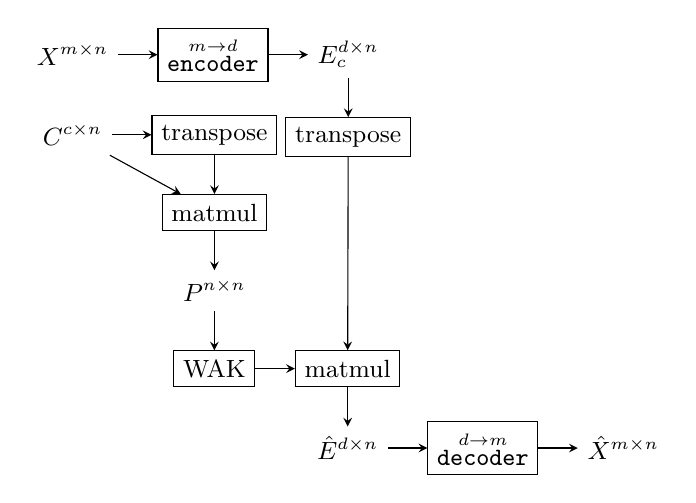
\begin{tikzpicture}[
    node distance = 5mm and 5mm,
    punkt/.style = {rectangle, draw},
    pil/.style = {black, -stealth},
    font=\small
    ]

  %\node[punkt] (preprocessing) {preprocessing} ;
  \node[] (X) {$X^{m \times n}$} ;
  \node[punkt] (encoder) [right=of X] {$\encoder^{m \to d}$} ;

  \node[] (E) [right=of encoder] {$E_c^{d \times n}$} ;
  \node[punkt] (Etranspose) [below=of E] {transpose} ;

  \node[] (C) [below=of X] {$C^{c \times n}$} ;
  \node[punkt] (Ctranspose) [right=of C] {transpose} ;
  \node[punkt] (CC) [below=of Ctranspose] {matmul} ;
  \node[] (P) [below=of CC] {$P^{n \times n}$} ;
  \node[punkt] (wak) [below=of P] {WAK} ;
  \node[punkt] (GE) [right=of wak] {matmul} ;
  \node[] (Ehat) [below=of GE] {$\hat{E}^{d \times n}$} ;

  \node[punkt] (decoder) [right=of Ehat] {$\decoder^{d \to m}$} ;
  \node[] (Xhat) [right=of decoder] {$\hat{X}^{m \times n}$} ;

  \draw[pil] %(preprocessing) edge (X)
  
  (X) edge (encoder)
  (encoder) edge (E)
  (E) edge (Etranspose)
  (Etranspose) edge (GE)

  (C) edge (Ctranspose)
  (Ctranspose) edge (CC)
  (C) edge (CC)
  (CC) edge (P)
  (P) edge (wak)
  (wak) edge (GE)
  (GE) edge (Ehat)

  (Ehat) edge (decoder)
  (decoder) edge (Xhat);
\end{tikzpicture}


         \caption{}
         \label{fig:}
     \end{subfigure}

     \caption{(a,b) Calculation of consensus $E$ and $C$, respectively.
     (c,d) Drop-in of consensus $E$ and $C$.}
     \label{fig:}
\end{figure}

\subsection{Recurrent DeePWAK}


\section{Results}

\subsection{Multihead DeePWAK learns sparse representations}

\begin{figure}
  %\begin{subfigure}[b]{0.5\textwidth}
  \includegraphics[width=\textwidth]{embeddings.pdf}
    \caption{DeePWAK learns sparse embedding values. }
    \label{fig:}
\end{figure}

    
\begin{figure}
  \includegraphics[width=\textwidth]{logits.pdf}
  \caption{For most heads, two clusters dominate.}
  \label{fig:}
\end{figure}

\begin{figure}
  \includegraphics[width=\textwidth]{phenotype.pdf}
  \caption{Hypergeometric test for enrichment of phenotype and treatment condition for each cluster in each head. Dot color indicates overrepresentation of each category in a cluster compared to a uniform prior. Dot size indicates statistical significance of the difference. Dot outline shade indicates number of embryos represented by a dot. Head 1 appears ``polysemantic''. The others appear to distinguish single phenotypic categories.}
  \label{fig:}
\end{figure}


\section{Discussion}

\subsection{Cluster-feature decomposition}
This striking result seems likely to be due to learning an embedding and partition of the data simultaneously.

\paragraph{Na\"ive Bayes interpretation}
For each minibatch forward pass, the partitioner gives a prior on each sample being in the same cluster.
During training it updates based on how well its classification does at predicting the data.

\paragraph{GCN interpretation}
A key insight of $\ntos$ is the unique power of generative processes.



\subsection{Application to sparse dictionary learning}

The embeddings appear to be representing the data as a sparse dictionary of features.
These features appear to match observable phenotypes.
Clusters are also sparse. However, \textit{there are more clusters than features}.
This is suggestive that data may be represented as \textit{combinatoric} mixtures of features. 

\subsection{The future of SAEs}

We suspect combinatoric encoding of this sort is possible because \DeePWAK performs computation on an entire minibatch.

\subsection{Insight into the unreasonable effectiveness of transformers}
\paragraph{$QK,OV$ decomposition}
\paragraph{Context matters even when there's no positional information}
\paragraph{Attention is graph diffusion}
\paragraph{Attention is $\ntos$}




\section{Conclusion}

\printbibliography

\end{document}
